\documentclass[12pt]{scrartcl}
\usepackage[sexy]{james}
\usepackage[noend]{algpseudocode}
\setlength{\marginparwidth}{2cm}
\usepackage{graphicx}
\usepackage{answers}
\usepackage{array}
\usepackage{tikz}
\newenvironment{allintypewriter}{\ttfamily}{\par}
\usepackage{listings}
\usepackage{xcolor}
\usetikzlibrary{arrows.meta}
\usepackage{color}
\usepackage{mathtools}
\newcommand{\U}{\mathcal{U}}
\newcommand{\E}{\mathbb{E}}
\usetikzlibrary{arrows}
\Newassociation{hint}{hintitem}{all-hints}
\renewcommand{\solutionextension}{out}
\renewenvironment{hintitem}[1]{\item[\bfseries #1.]}{}
\renewcommand{\O}{\mathcal{O}}
\declaretheorem[style=thmbluebox,name={Chinese Remainder Theorem}]{CRT}
\renewcommand{\theCRT}{\Alph{CRT}}
\setlength\parindent{0pt}
\usepackage{sansmath}
\usepackage{pgfplots}

\usetikzlibrary{automata}
\usetikzlibrary{positioning}  %                 ...positioning nodes
\usetikzlibrary{arrows}       %                 ...customizing arrows
\newcommand{\eqdef}{=\vcentcolon}
\newcommand{\tr}{{\rm tr\ }}
\newcommand{\im}{{\rm Im\ }}
\newcommand{\spann}{{\rm span\ }}
\newcommand{\Col}{{\rm Col\ }}
\newcommand{\Row}{{\rm Row\ }}
\newcommand{\dint}{\displaystyle\int}
\newcommand{\dt}{\ {\rm d }t}
\newcommand{\PP}{\mathbb{P}}
\newcommand{\horizontal}{\par\noindent\rule{\textwidth}{0.4pt}}
\usepackage[top=3cm,left=3cm,right=3cm,bottom=3cm]{geometry}
\newcommand{\mref}[3][red]{\hypersetup{linkcolor=#1}\cref{#2}{#3}\hypersetup{linkcolor=blue}}%<<<changed

\tikzset{node distance=4.5cm, % Minimum distance between two nodes. Change if necessary.
         every state/.style={ % Sets the properties for each state
           semithick,
           fill=cyan!40},
         initial text={},     % No label on start arrow
         double distance=4pt, % Adjust appearance of accept states
         every edge/.style={  % Sets the properties for each transition
         draw,
           ->,>=stealth',     % Makes edges directed with bold arrowheads
           auto,
           semithick}}


% Start of document.
\newcommand{\sep}{\hspace*{.5em}}

\pgfplotsset{compat=1.18}
\begin{document}
\title{MATH410: Homework 3}
\author{James Zhang\thanks{Email: \mailto{jzhang72@terpmail.umd.edu}}}
\date{\today}

\definecolor{dkgreen}{rgb}{0,0.6,0}
\definecolor{gray}{rgb}{0.5,0.5,0.5}
\definecolor{mauve}{rgb}{0.58,0,0.82}

\lstset{frame=tb,
  language=Java,
  aboveskip=3mm,
  belowskip=3mm,
  showstringspaces=false,
  columns=flexible,
  basicstyle={\small\ttfamily},
  numbers=left,
  numberstyle=\tiny\color{gray},
  keywordstyle=\color{blue},
  commentstyle=\color{dkgreen},
  stringstyle=\color{mauve},
  breaklines=true,
  breakatwhitespace=true,
  tabsize=3
}

\maketitle

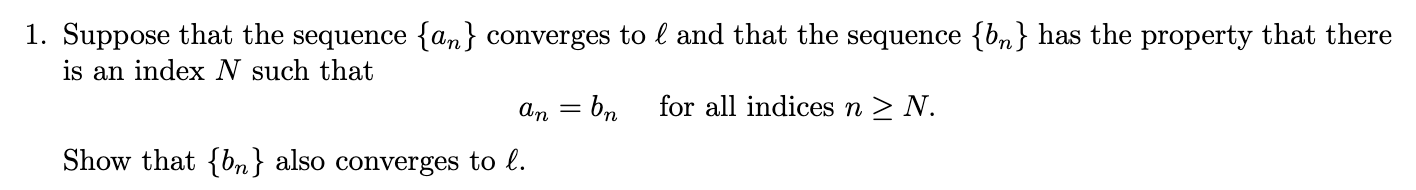
\includegraphics[width=15cm]{1.png}

\begin{proof}
  
\hfill

On the contrary, assume that a strictly increasing sequence $\{a_n\}$ has a peak index $a_m$, for some 
$m \in \NN$. By definition of strictly increasing, $a_{n+1} \geq a_n \ \forall \ n \in \NN$.
Since this works for all $n$, note that by definition of strictly increasing, $a_{m+1} \geq m$.
However, note that by definition of peak index
\[a_m > a_j \ \forall \ j \geq m \implies a_m > a_{m+1}\]
Thus, we've reached a contradiction since $a_{m+1} \geq m$ and $a_{m+1} < m$ obviously cannot
both be simulatenously true.
\end{proof}

\newpage

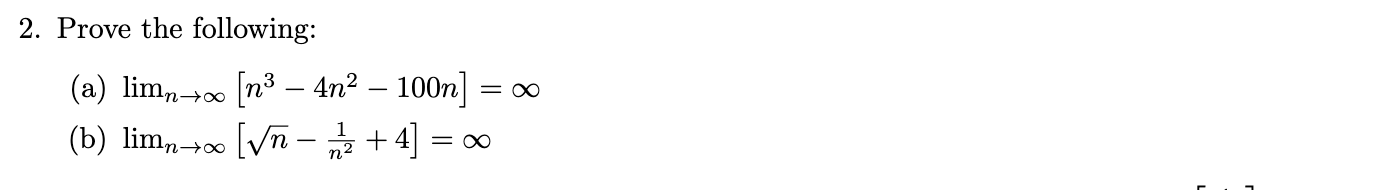
\includegraphics[width=15cm]{2.png}

\begin{proof}
  
\hfill

$\Longrightarrow$ Suppose we are given that the sequence $\{a_n\}$ does not converge to the 
number $a$. Therefore, by the definition of convergence, given some $\epsilon > 0$, 
we are not always guaranteed to be able to find $N \in \NN$ such that 
\[|a_n - a| < \epsilon \ \forall \ n \geq N\]
Choose one of these examples of $\epsilon$. Let us define the monotonically increasing sequence 
$\{n_k\} = \{i \ | \ |a_i - a| \geq \epsilon, i \geq N, i \in \NN\}$, or in plain English, all indices $i \geq N$
such that $|a_i - a| \geq \epsilon$.
Therefore, we have constructed a subsequence $\{a_{n_k}\}$ such that 
\[|a_{n_k} - a| \geq \epsilon \ \forall \ k\]
as desired.

\hfill

$\Longleftarrow$ The reverse direction is similar. Given $\epsilon > 0$ and some subsequence $\{a_{n_k}\}$, 
\[|a_{n_k} - a| \geq \epsilon \ \forall \ k\]
We WTS that $\{a_n\}$ does not converge to $a$. Suppose on the contrary, $\{a_n\}$ did converge to $a$. 
By definition of convergence, given any $\epsilon > 0$, we can find threshold $N \in \NN$ such that 
\[|a_n - a| < \epsilon \ \forall \ n \geq N\]
Note that this definition should work for all $\epsilon > 0$. Therefore,
let us choose the same $\epsilon$ as in the given statement. Note that $\{n_k\}$ is a monotonically increasing infinite sequence 
of natural numbers by definition of subsequence. Therefore, there exists some index in $\{n_k\}$ that is greater than or equal to
our threshold $N$. Let us denote this index $x$. Therefore, at index $x$, we have that $|a_x - a| \geq \epsilon$ by the given and $|a_x - a| < \epsilon$ by the definition of convergence. Clearly, this is a contradiction, 
and so $\{a_n\}$ cannot converge to $a$. 

\end{proof}

\newpage

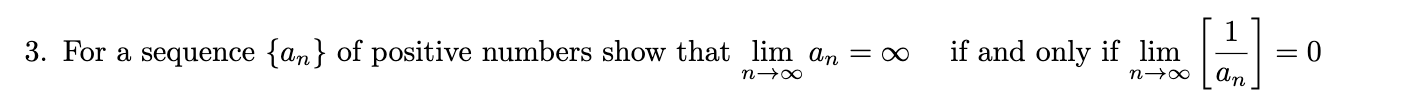
\includegraphics[width=15cm]{3.png}

\begin{proof}[Solution]

\hfill

\begin{enumerate}[a.]
  \item True. Assume on the contradiction that a bounded sequence $\{a_n\}$ had an unbounded subsequence $\{a_{n_k}\}$. 
  By definition of bounded, $\exists \ M \in \RR$ such that $|a_n| < M \ \forall \ n \implies -M < a_n < M \ \forall \ n$.
  If subsequence $\{a_{n_k}\}$ is unbounded then there some there exists some index $x \in \{n_k\}$ such that 
  $|a_x| \geq M$ because no scalar, not even $M$, is greater than the absolute value of all elements in the subsequence. 
  However $a_x$ is in the subsequence and also the sequence, so we have $|a_x| < M$ and $|a_x| \geq M$ simulatenously, which
  must be a contradiction, and so $\{a_{n_k}\}$ must also be bounded.
  \item True. 
  \item True.
  \item False. Consider the sequence $\{a_n\} = \{\frac{1}{n}\}$ and the subsequent subsequence 
  $\{a_{n_k}\} = \{\frac{1}{n} \ | \ n \text{ is even}\}$. Note that $\{a_{n_k}\}$ converges to $1$, 
  but that the original subsequence we know does not converge. Therefore, we've found a counterexample.
\end{enumerate}
  
\end{proof}

\newpage

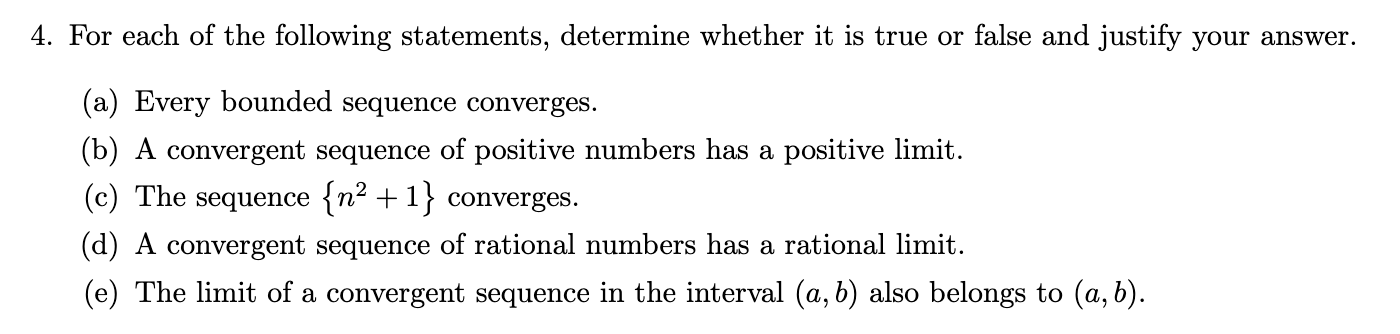
\includegraphics[width=15cm]{4.png}

\begin{proof}
  
\hfill


\end{proof}
\newpage

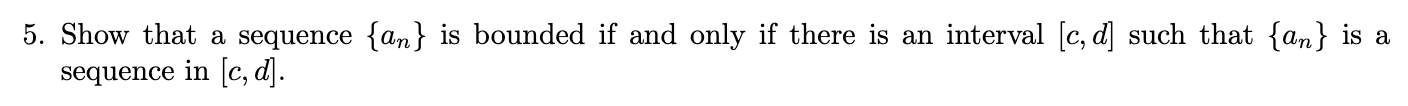
\includegraphics[width=15cm]{5.png}

\begin{proof}
  
\hfill


\end{proof}
\newpage

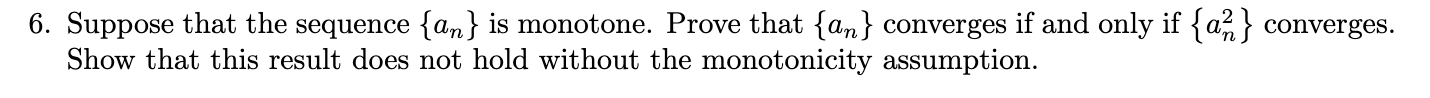
\includegraphics[width=15cm]{6.png}

\begin{proof}
  
\hfill


\end{proof}
\newpage

\includegraphics[width=15cm]{7.png}

\begin{proof}
  
\hfill


\end{proof}
\newpage

\includegraphics[width=15cm]{8.png}

\begin{proof}
  
\hfill


\end{proof}
\end{document}

